\documentclass[tikz,border=4pt]{standalone}
\usepackage[T1]{fontenc}
\usepackage{lmodern}
\usepackage{xcolor}
\usetikzlibrary{arrows.meta,positioning,calc}

\definecolor{vbteal}{RGB}{94,170,160}
\definecolor{vbgray}{RGB}{110,110,110}

\begin{document}
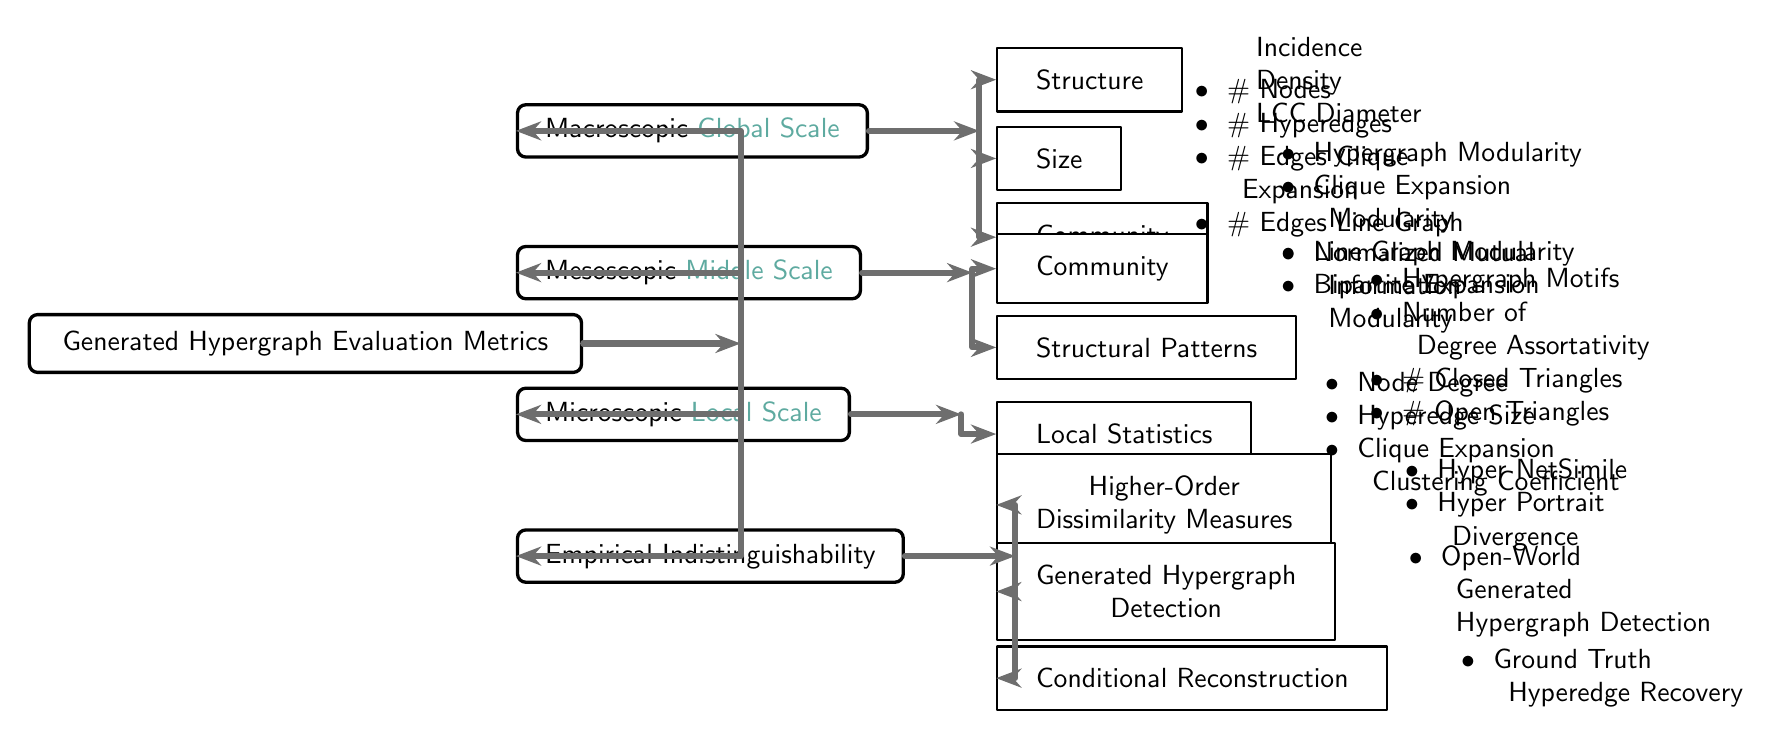
\begin{tikzpicture}[
  font=\sffamily,
  >=Stealth,
  line cap=round,
  line join=round,
  header/.style={draw=black, rounded corners=3pt, very thick, fill=white, inner xsep=12pt, inner ysep=6pt},
  cat/.style   ={draw=black, rounded corners=3pt, very thick, fill=white, inner xsep=10pt, inner ysep=5pt},
  sub/.style   ={draw=black, thick, fill=white, inner xsep=14pt, inner ysep=8pt, align=center},
  conn/.style  ={draw=vbgray, line width=2.2pt, -{Stealth[length=3.2mm,width=2.4mm]}}
]

% ---------------- Root (LEFT) ----------------
\node[header, anchor=west] (T) at (0,0) {Generated Hypergraph Evaluation Metrics};

% A vertical "spine" of category nodes to the RIGHT of the root
\node[cat, anchor=west] (MAC) at (6.2,  2.7) {Macroscopic \textcolor{vbteal}{Global Scale}};
\node[cat, anchor=west] (MES) at (6.2,  0.9) {Mesoscopic \textcolor{vbteal}{Middle Scale}};
\node[cat, anchor=west] (MIC) at (6.2, -0.9) {Microscopic \textcolor{vbteal}{Local Scale}};
\node[cat, anchor=west] (EMP) at (6.2, -2.7) {Empirical Indistinguishability};

% Connector from root to a hub, then to each category (like a horizontal fan-out)
\coordinate (hub) at ($(T.east)+(2.0,0)$);
\draw[conn] (T.east) -- (hub);
\draw[conn] (hub) |- (MAC.west);
\draw[conn] (hub) |- (MES.west);
\draw[conn] (hub) |- (MIC.west);
\draw[conn] (hub) |- (EMP.west);

% ---------------- Macroscopic sub-blocks ----------------
\node[sub, anchor=west] (S1) at (12.3, 3.35) {Structure};
\node[sub, anchor=west] (S2) at (12.3, 2.35) {Size};
\node[sub, anchor=west] (S3) at (12.3, 1.35) {Community};

\coordinate (mhub) at ($(MAC.east)+(1.4,0)$);
\draw[conn] (MAC.east) -- (mhub);
\draw[conn] (mhub) |- (S1.west);
\draw[conn] (mhub) |- (S2.west);
\draw[conn] (mhub) |- (S3.west);

\node[anchor=west, align=left] at ($(S1.east)+(0.8,0)$) {%
Incidence\\
Density\\
LCC Diameter%
};
\node[anchor=west, align=left] at ($(S2.east)+(0.8,0)$) {%
$\bullet$ \ \# Nodes\\
$\bullet$ \ \# Hyperedges\\
$\bullet$ \ \# Edges Clique\\
\hspace*{1.7em}Expansion\\
$\bullet$ \ \# Edges Line Graph%
};
\node[anchor=west, align=left] at ($(S3.east)+(0.8,0)$) {%
$\bullet$ \ Hypergraph Modularity\\
$\bullet$ \ Clique Expansion\\
\hspace*{1.7em}Modularity\\
$\bullet$ \ Line Graph Modularity\\
$\bullet$ \ Bipartite Expansion\\
\hspace*{1.7em}Modularity%
};

% ---------------- Mesoscopic sub-blocks ----------------
\node[sub, anchor=west] (M1) at (12.3, 0.95) {Community};
\node[sub, anchor=west] (M2) at (12.3,-0.05) {Structural Patterns};

\coordinate (meshb) at ($(MES.east)+(1.4,0)$);
\draw[conn] (MES.east) -- (meshb);
\draw[conn] (meshb) |- (M1.west);
\draw[conn] (meshb) |- (M2.west);

\node[anchor=west, align=left] at ($(M1.east)+(0.8,0)$) {%
$\bullet$ \ Normalized Mutual\\
\hspace*{1.7em}Information%
};
\node[anchor=west, align=left] at ($(M2.east)+(0.8,0)$) {%
$\bullet$ \ Hypergraph Motifs\\
$\bullet$ \ Number of\\
\hspace*{1.7em}Degree Assortativity\\
$\bullet$ \ \# Closed Triangles\\
$\bullet$ \ \# Open Triangles%
};

% ---------------- Microscopic sub-blocks ----------------
\node[sub, anchor=west] (L1) at (12.3,-1.15) {Local Statistics};

\coordinate (lichb) at ($(MIC.east)+(1.4,0)$);
\draw[conn] (MIC.east) -- (lichb);
\draw[conn] (lichb) |- (L1.west);

\node[anchor=west, align=left] at ($(L1.east)+(0.8,0)$) {%
$\bullet$ \ Node Degree\\
$\bullet$ \ Hyperedge Size\\
$\bullet$ \ Clique Expansion\\
\hspace*{1.7em}Clustering Coefficient%
};

% ---------------- Empirical sub-blocks ----------------
\node[sub, anchor=west] (E1) at (12.3,-2.05) {Higher-Order\\Dissimilarity Measures};
\node[sub, anchor=west] (E2) at (12.3,-3.15) {Generated Hypergraph\\Detection};
\node[sub, anchor=west] (E3) at (12.3,-4.25) {Conditional Reconstruction};

\coordinate (emphb) at ($(EMP.east)+(1.4,0)$);
\draw[conn] (EMP.east) -- (emphb);
\draw[conn] (emphb) |- (E1.west);
\draw[conn] (emphb) |- (E2.west);
\draw[conn] (emphb) |- (E3.west);

\node[anchor=west, align=left] at ($(E1.east)+(0.8,0)$) {%
$\bullet$ \ Hyper NetSimile\\
$\bullet$ \ Hyper Portrait\\
\hspace*{1.7em}Divergence%
};
\node[anchor=west, align=left] at ($(E2.east)+(0.8,0)$) {%
$\bullet$ \ Open-World\\
\hspace*{1.7em}Generated\\
\hspace*{1.7em}Hypergraph Detection%
};
\node[anchor=west, align=left] at ($(E3.east)+(0.8,0)$) {%
$\bullet$ \ Ground Truth\\
\hspace*{1.7em}Hyperedge Recovery%
};

\end{tikzpicture}
\end{document}